%% ISAE-SUPAERO report template for research projects 
%% V1.0
%% 2016/04/14
%% by Damien Roque
%% See http://personnel.isae.fr/damien-roque


%% This template is based on bare_conf.tex
%% V1.4b
%% 2015/08/26
%% by Michael Shell

%%*************************************************************************
%% Legal Notice:
%% This code is offered as-is without any warranty either expressed or
%% implied; without even the implied warranty of MERCHANTABILITY or
%% FITNESS FOR A PARTICULAR PURPOSE! 
%% User assumes all risk.
%% In no event shall the IEEE or any contributor to this code be liable for
%% any damages or losses, including, but not limited to, incidental,
%% consequential, or any other damages, resulting from the use or misuse
%% of any information contained here.
%%
%% All comments are the opinions of their respective authors and are not
%% necessarily endorsed by the IEEE.
%%
%% This work is distributed under the LaTeX Project Public License (LPPL)
%% ( http://www.latex-project.org/ ) version 1.3, and may be freely used,
%% distributed and modified. A copy of the LPPL, version 1.3, is included
%% in the base LaTeX documentation of all distributions of LaTeX released
%% 2003/12/01 or later.
%% Retain all contribution notices and credits.
%% ** Modified files should be clearly indicated as such, including  **
%% ** renaming them and changing author support contact information. **
%%*************************************************************************

\documentclass[conference]{IEEEtran}

\usepackage[utf8]{inputenc}
\usepackage{ifthen}
\usepackage[backend=biber, style=ieee]{biblatex}
\addbibresource{references_final_report.bib}
\usepackage{hyperref}
\usepackage{url}
\usepackage[pdftex]{graphicx}
\graphicspath{{images/}}
\usepackage{tikz,filecontents}
\usetikzlibrary{matrix,calc}
\usetikzlibrary{shapes,arrows,shadings,patterns}
\usepackage{pgfplots}
\pgfplotsset{compat=newest}
\pgfplotsset{plot coordinates/math parser=false}
\newlength\figureheight
\newlength\figurewidth

\usepackage{amsfonts}
\usepackage[cmex10]{amsmath}
\usepackage{multirow}
\usepackage[acronym,indexonlyfirst,nomain]{glossaries}

% Examples of several macros
\newcommand*{\SET}[1]{\ensuremath{\boldsymbol{#1}}}
\newcommand*{\VEC}[1]{\ensuremath{\boldsymbol{\mathrm{#1}}}}
\newcommand*{\FAM}[1]{\ensuremath{\mathrm{#1}}}
\newcommand*{\MAT}[1]{\ensuremath{\boldsymbol{\mathrm{#1}}}}
\newcommand*{\OP}[1]{\ensuremath{\mathrm{#1}}}
\newcommand*{\NORM}[1]{\ensuremath{\left\|#1\right\|}}
\newcommand*{\DPR}[2]{\ensuremath{\left \langle #1,#2 \right \rangle}}

\newtheorem{theorem}{Theorem}

\newcommand{\alert}[1]{\textcolor{red}{#1}}
\usepackage[caption=false,font=footnotesize]{subfig}

% correct bad hyphenation here
\hyphenation{op-tical net-works semi-conduc-tor}


\begin{document}
%
% paper title
% Titles are generally capitalized except for words such as a, an, and, as,
% at, but, by, for, in, nor, of, on, or, the, to and up, which are usually
% not capitalized unless they are the first or last word of the title.
% Linebreaks \\ can be used within to get better formatting as desired.
% Do not put math or special symbols in the title.
\title{REMAINING USEFUL LIFE PREDICTIONS WITH DEEP LEARNING METHODS}

% for over three affiliations, or if they all won't fit within the width
% of the page, use this alternative format:
% 
\author{\IEEEauthorblockN{Thomas Guillebot de Nerville\IEEEauthorrefmark{1},
Paul Strähle\IEEEauthorrefmark{1},
Anass Akrim\IEEEauthorrefmark{2}\IEEEauthorrefmark{3} and 
Rob Vingerhoeds\IEEEauthorrefmark{2}}

\IEEEauthorblockA{\IEEEauthorrefmark{1}Institut Supérieur de l'Aéronautique et de l'Espace (ISAE-SUPAERO), Université de Toulouse, 31400 Toulouse, FRANCE\\
Email: \{thomas.guillebot-de-nerville,paul.strahle\}@student.isae-supaero.fr}
\IEEEauthorblockA{\IEEEauthorrefmark{2}Institut Supérieur de l'Aéronautique et de l'Espace (ISAE-SUPAERO), Université de Toulouse, 31400 Toulouse, FRANCE\\
Email: \{anass.akrim,rob.vingerhoeds\}@isae-supaero.fr}
\IEEEauthorblockA{\IEEEauthorrefmark{3}Institut Clément Ader (UMR CNRS 5312) INSA/UPS/ISAE/Mines Albi, Université de Toulouse, 31400 Toulouse, FRANCE\\
Email: anass.akrim@univ-tlse3.fr}
}


%\IEEEspecialpapernotice{(Bibliography report)}
\IEEEspecialpapernotice{(Final report)}

% import the acronyms
% Here are the acronyms
\newacronym{nlp}{NLP}{Natural Language Processing}
\newacronym{phm}{PHM}{Prognostics and Health Management}
\newacronym{rul}{RUL}{Remaining Useful Life}
\newacronym{rnn}{RNN}{Recurrent Neural Network}
\newacronym{lstm}{LSTM}{Long short-term memory}
\newacronym{gru}{GRU}{Gated Recurrent Unit}
\newacronym{cnn}{CNN}{Convolutional Neural Network}
\newacronym{tcn}{TCN}{Temporal Convolutional Network}
\newacronym{erm}{ERM}{Elman Recurrent Network}
\newacronym{mlp}{MLP}{Machine Learning Program}
\newacronym{lrdecay)}{lrDecay)}{learning rate decay}

% make the title area
\maketitle

% As a general rule, do not put math, special symbols or citations
% in the abstract
\begin{abstract}

This paper aims to compare Deep Learning models to predict the \gls{rul} of a structure. The investigated models are the following: the \gls{cnn} family with the 1D-\gls{cnn} and \gls{tcn} architectures and the \gls{rnn} family with the \gls{rnn}, \glspl{lstm} and \glspl{gru} architectures.

The dataset for training and testing consists in simulations of the crack growth in plates, based on the Paris-Erdogan law. The training and validation dataset is composed of 10\,000 structures while the testing dataset is composed of 100 structures. Each architecture is optimized and trained on respectively 100, 500 and 1000 structures from the training dataset. At the end, the different models are evaluated and compared on the testing dataset on the basis of the accuracy metric.

In order to optimize the architectures, the first step is to identify the fixed parameters which do not have a significant impact on the accuracy, and the variable ones which should be optimized. The variable hyperparameters are optimized with a Random Search Strategy on 100 and 500 structures for the \gls{rnn} family. For the \gls{cnn} family, the models are optimized on 100, 500 and 1000 structures. The optimized models are then fine tuned with an adaptive learning rate. The results show that within the \gls{rnn} family \glspl{gru} make the best predictions while within the \gls{cnn} family \glspl{tcn} do so.

Both the \gls{gru} and \gls{tcn} models show a validation accuracy of greater than 95\% when trained on 500 or 1000 structures. But the \gls{tcn} outperforms all other models on the testing dataset where it reaches 99\% accuracy after being trained on 1000 structures.

All results of this study as well as the created code is available publicly at \url{https://github.com/blitzpaal/RUL-Prediction}.

\end{abstract}

\IEEEpeerreviewmaketitle

\section{Background}
\label{sec:background}

\subsection{Deep Learning}

In recent years Deep Learning, a subbranch of Machine Learning, has shown impressive results, especially in the fields of speech recognition, visual object recognition and object detection \cite{LeCun2015}. One requirement in using Deep Learning is the presence of sufficient amounts of data \cite{Sikorska2011}. As more data becomes available in the engineering domain there is a recent surge of interest in using Deep Learning in engineering \cite{Voulodimos2018}.

One of the strengths of Deep Learning approaches is their ability to deal with and detect complex relationships in large datasets \cite{MONTEROJIMENEZ2020539}. This strength makes their usage also interesting in the \gls{phm} domain \cite{Wu2015}. The potential of Deep Learning in \gls{phm} might not be fully exploited yet \cite{Akrim2021}.

\subsection{Prognostics and Health Management}

According to Zio \cite{Zio2012} \gls{phm} is a field of research and application which aims at making use of past, present and future information on the environmental, operational and usage conditions of a piece of equipment in order to detect its degradation, diagnose its faults, predict and proactively manage its failures. In the context of this project only the detection of degradation and prediction of failure are relevant.

\gls{phm} models can be divided into single and multi-model approaches. Multi-model approaches are a combination of different single-model approaches. Single-model approaches can be further divided into knowledge-based, data-driven and physics-based models. Within the data-driven models there are statistical, stochastic and Machine Learning models which is the category of Deep Learning models. \cite{MONTEROJIMENEZ2020539}

\section{Interest}
\label{sec:interest}

Deep Learning has shown some impressive results when applied to \gls{rul} prediction as shown in \cite{Xu2018, Li2018, Liu2019, Yuan2016, Wu2018, Park2020} and other publications (For an overview see Akrim et al. \cite{Akrim2021}).

Within the available Deep Learning models there are two algorithms which are promising for \gls{rul} prediction: \glspl{rnn} (Little \cite{Little1996} and Hopfield  \cite{Hopfield1982}) and \glspl{cnn} (Lecun et al. \cite{Lecun1998}) \cite{Akrim2021}.

\glspl{rnn} are the common Deep Learning approach for time-dependent relationships and have therefore also achieved great interest in the \gls{phm} domain \cite{Akrim2021}. Pioneering models were developed such as \glspl{erm} \cite{Elman1990} or Jordan Networks \cite{Jordan1997}, outperforming traditional \glspl{mlp} for sequence-prediction \cite{Akrim2021}. These algorithms were then widely explored by several researchers. Among them can be cited Yan et al. \cite{Yan2007} for their work on material degradation evaluation and life prediction in 2007, and Kramti et al. \cite{Kramti2018} for having used \glspl{erm} for high-speed shaft bearing prognostics based on vibration signals \cite{Akrim2021}.

An emerging type of Deep Learning network for time-dependent relationships are \glspl{cnn} which might be able to outperform \glspl{rnn} \cite{Bai2018}. In one of the first applications of \glspl{cnn} to \gls{phm} Li et al. suggested that \glspl{cnn} can be used to obtain \gls{rul} prognoses for machinery \cite{Li2018}. The model was applied to the C-MAPSS dataset \cite{Saxena2008} and outperformed state-of-the-art prognostics approaches including \gls{rnn} and \gls{lstm} models.

In this work a synthetic dataset is used as according to Fink et al. \cite{Fink2020} the use of simulation environments and adaption to real-life applications is a promising future research approach as the data will more likely be sufficient in the source domain. The synthetic dataset used for this study aims at using this advantage.

The synthetic dataset matches strain gauge data to \gls{rul} values. The use of strain gauges as an input to a \gls{phm} model is interesting as they play a vital role in \gls{phm} in general \cite{Tinga2019} and specifically for the aircraft domain \cite{Timothy2009}.

\section{Aim}
\label{sec:aim}

The aim of this study is to predict the \gls{rul} of precracked plates based on strain gauge measurements using Deep Learning. 
For the application of Deep Learning to crack growth for \gls{rul} prediction based on strain gauge measurements no relevant results in the literature could be found. This study attempts to fill this research gap.

In a work done by Akrim \cite{Akrim} the Paris-Erdogan Law \cite{Paris1963} was used to create a synthetic dataset of crack growth to train the model. The dataset consists of strain data from virtual strain gauges placed in the area around the crack and the corresponding \gls{rul} of the plates.

The Paris-Erdogan Law is applied to an infinite plate with a central horizontal crack. The strain gauges are placed in a 45°-Angle at the positions shown in Figure \ref{fig:strain_gauge_positions} relative to the center of the plate where the crack is located.

\begin{figure}[htp]
	\centering
	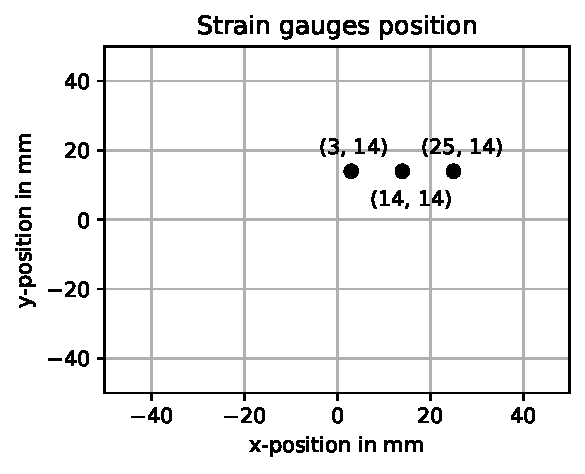
\includegraphics[width=6cm]{python/strain_gauges_position.pdf}
	\caption{Position of the strain gauges relative to the crack}
	\label{fig:strain_gauge_positions}
\end{figure}

The crack length in the Paris-Erdogan Law is a function of the number of cylces $k$, stress range $\Delta \sigma$, material constants $m, C$ and initial crack length $a_0$. By calculating the crack growth until the crack length $a$ reaches the critical crack length $a_{crit}=(\frac{K_{IC}}{\Delta \sigma \sqrt{\pi}})^2$ the simulation can determine the \gls{rul} for each simulated cycle. For the simulations the stress range $\Delta \sigma$ is kept constant while the initial crack length $a_0$ and the material parameters $m$ and $C$ are drawn from a normal distribution. $ 10\,000 $ structures are generated this way to form the training and validation datasets. For the testing dataset 100 structures are generated. The output of these simulations which forms the input and output for the Deep Learning models is a table matching the strains from the strain gauges to the \gls{rul}. To reduce the dataset the results are only saved to the table every 500 cycles. Table \ref{tab:sliding_window_approach} shows the structure of the generated training and validation dataset. The label $ ID $ denotes the specific structure.

\begin{table}[htp]
	\centering
	\caption{Training and validation dataset structure}
	\label{tab:sliding_window_approach}
	\begin{tabular}{lllllll}
		$ \boldsymbol{t} $ & $ \boldsymbol{ID} $ & $ \boldsymbol{cycle} $ & $ \boldsymbol{\epsilon_1} $     & $ \boldsymbol{\epsilon_2} $     & $ \boldsymbol{\epsilon_3} $     & $ \boldsymbol{RUL} $   \\
		\hline
		$ 1 $ & $ 1 $  & $ 0 $     & $ \epsilon_{1,1} $ & $ \epsilon_{2,1} $ &  $ \epsilon_{3,1} $ &  $ RUL_1 $ \\
		$ 2 $ & $ 1 $  & $ 500 $   & $ \epsilon_{1,2} $ & $ \epsilon_{2,2} $ & $ \epsilon_{3,2} $ & $ RUL_2 $ \\
		$ 3 $ & $ 1 $  & $ 1000 $  & $ \epsilon_{1,3} $ & $ \epsilon_{2,3} $ & $ \epsilon_{3,3} $ & $ RUL_3 $ \\
		$ 4 $ & $ 1 $  & $ 1500 $  & $ \epsilon_{1,4} $ & $ \epsilon_{2,4} $ & $ \epsilon_{3,4} $ & $ RUL_4 $ \\
		\vdots & \vdots & \vdots & \vdots & \vdots &\vdots & \vdots \\
		$ n $ & $ 10000 $  & $ N_{f,10000} $  & $ \epsilon_{1,5} $ & $ \epsilon_{2,5} $ & $ \epsilon_{3,5} $ & $ RUL_5 $
	\end{tabular}
\end{table}

The aim of this work is to predict the \gls{rul} based on current and past information from the 3 strain gauges time series using Deep Learning models. Different Deep Learning model architectures are to be used for that. The developed models should be trained and optimized before a comparison between them is made.

\section{Methods}
\label{sec:methods}

\subsection{Available Dataset}
\label{sec:available_dataset}

The created training and validation dataset with $ 10\,000 $ structures is divided into different subsets for training and validation. The last $ 100 $ structures of the training dataset are always used as the validation dataset. For training either the first $ 100 $, $ 500 $ or $ 1000 $ structures are used. One training run with the \gls{tcn} architecture is performed using $ 9\,900 $ structures for training and therefore using the full dataset for training and validation. For testing the models always the same testing dataset with $ 100 $ structures is used.

As it showed promising results in other applications of Deep Learning to \gls{phm} (\cite{Liu2019a, Xiao2016}), classification is an interesting alternative to regression for \gls{rul} prediction. Instead of trying to predict an exact \gls{rul} value the goal is to predict the correct \gls{rul} class with a lower and upper bound for the \gls{rul}. The structures in the generated dataset have a \gls{rul} value of around $ 80\,000 $ cycles at most. Therefore the chosen strategy is to create $ 19 $ intervals following a parabolic equation between $ 0 $ and $ 80\,000 $ cycles. Figure \ref{fig:RNN_classification} shows the principal output of the neural networks as well as the boundaries between the \gls{rul} classes. After the $ 19 $ classes following the parabolic equation a last class is added for all \gls{rul} values greater than $ 80\,000 $ cycles. The total number of classes is therefore $ C = 20 $. The reason to use the parabolic equation for class generation is to generate more classes near a \gls{rul} value near $ 0 $ as it is more critical to generate accurate predictions near the failure of the structures.

\begin{figure}[htp]
	\centering
	\subfloat[][]{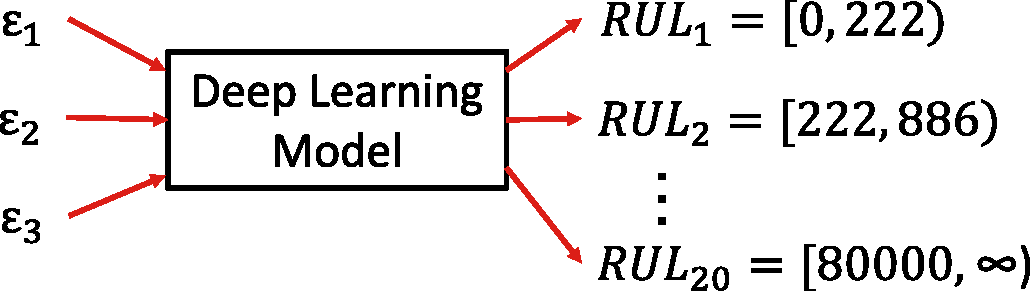
\includegraphics[width=0.35\textwidth]{classification_model.pdf}}
	\\
	\subfloat[][]{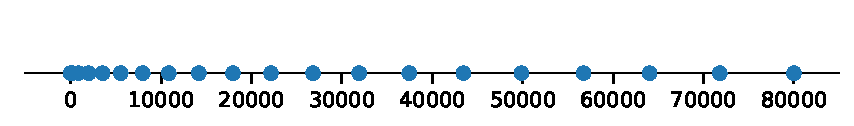
\includegraphics[width=0.45\textwidth]{python/RUL_classification.pdf}}
	\caption{(a): Neural network model output for \gls{rul} classification, (b): Boundaries between the \gls{rul} classes (The dots represent the boundaries)}
	\label{fig:RNN_classification}
\end{figure}

To prepare the data as an input and output for the networks a sliding window approach is used. This approach maps the \gls{rul} at time $ t $ onto the current and past time steps of the input features $ [x_{t-N+1}, x_{t-N+2},..., x_{t-1}, x_t] $ where $ N $ is the length of the sliding window. The resulting input matrix therefore has the dimension $ (n-N) \times N \times k $ where $ n $ is the number of samples and $ k $ is the number of features. Figure \ref{fig:input_matrix} shows an example of how the time series data of the strain gauges from Table \ref{tab:sliding_window_approach} is mapped to the input matrix.

\begin{figure}[htp]
	\centering
	\def\getangle(#1)(#2)#3{%
	\begingroup%
	\pgftransformreset%
	\pgfmathanglebetweenpoints{\pgfpointanchor{#1}{center}}{\pgfpointanchor{#2}{center}}%
	\expandafter\xdef\csname angle#3\endcsname{\pgfmathresult}%
	\endgroup%
}

\begin{tikzpicture}[every node/.style={anchor=north east,fill=white,minimum width=1.3cm,minimum height=6mm}]
	\matrix (mA) [draw,matrix of math nodes]
	{
		\epsilon_{3,1} & \epsilon_{3,2} &  \cdots &  \epsilon_{3,N}  \\
		\epsilon_{3,2}  &  \epsilon_{3,3}  &  \cdots &  \epsilon_{3,N+1}  \\
			\vdots          	& \vdots          	& \ddots & \vdots \\
		\epsilon_{3,n-N+1}  &  \epsilon_{3,n-N}  &  \cdots &  \epsilon_{3,n}  \\
	};
	\matrix (mB) [draw,matrix of math nodes] at ($(mA.south west)+(4.9,1.65)$)
	{
		 \epsilon_{2,1}  &  \epsilon_{2,2}  & \cdots &  \epsilon_{2,N}  \\
		 \epsilon_{2,2}  &  \epsilon_{2,3}  &  \cdots &  \epsilon_{2,N+1}  \\
		\vdots             & \vdots          	& \ddots & \vdots \\
		 \epsilon_{2,n-N+1}  &  \epsilon_{2,n-N}  &  \cdots &  \epsilon_{2,n}  \\
	};
	\matrix (mC) [draw,matrix of math nodes] at ($(mB.south west)+(4.9,1.65)$)
	{
		 \epsilon_{1,1}  &  \epsilon_{1,2}  &  \cdots &  \epsilon_{1,N}  \\
		 \epsilon_{1,2}  &  \epsilon_{1,3}  &  \cdots &  \epsilon_{1,N+1}  \\
		\vdots             & \vdots          	& \ddots 	  & \vdots \\
		 \epsilon_{1,n-N+1}  &  \epsilon_{1,n-N}  &  \cdots &  \epsilon_{1,n}  \\
	};

	\draw[dashed](mA.north east)--(mC.north east);
	\draw[dashed](mA.north west)--(mC.north west);
	\draw[dashed](mA.south east)--(mC.south east);
	
	\coordinate (A) at (mC.south east);
	\coordinate (B) at (mA.south east);
	\getangle(A)(B)a;
	\draw[thick,-stealth] ([xshift=2ex]mC.south east) -- ([xshift=2ex]mA.south east) node[midway,below,rotate=\anglea] {Number of features $ k $};
	\draw[thick,-stealth] ([yshift=-2ex]mC.south west) -- 
	([yshift=-2ex]mC.south east) node[midway,below] {Sliding window length $ N $};
	\draw[thick,-stealth] ([xshift=-2ex]mC.north west)
	-- ([xshift=-2ex]mC.south west) node[midway,above,rotate=90] {Time steps $ n $};
\end{tikzpicture}
	\caption{Input matrix for the neural networks}
	\label{fig:input_matrix}
\end{figure}

The output matrix shown in Figure \ref{fig:output_matrix} is only one dimensional. It is only composed of the \gls{rul} classes which are mapped to the corresponding rows in the input matrix. The dimension of the output matrix therefore is $ (n-N) $.

\begin{figure}[htp]
	\centering
	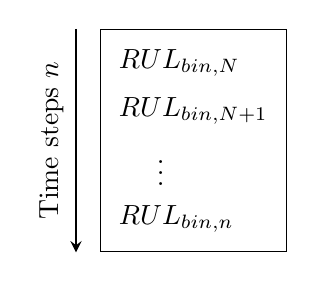
\begin{tikzpicture}[every node/.style={anchor=north west,fill=white,minimum width=1.3cm,minimum height=6mm}]
	\matrix (mA) [draw,matrix of math nodes]
	{
		RUL_{bin,N} \\
		RUL_{bin,N+1} \\
		\vdots \\
		RUL_{bin,n} \\
	};

	\draw[thick,-stealth] ([xshift=-2ex]mA.north west)
	-- ([xshift=-2ex]mA.south west) node[midway,above,rotate=90] {Time steps $ n $};
\end{tikzpicture}
	\caption{Output matrix for the neural networks}
	\label{fig:output_matrix}
\end{figure}

As an input for the different models, the datasets are normalized. While a specific layer is added at the beginning of the 1D-\gls{cnn} architecture to do so, the preprocessed data has to be normalized before being fed into the different \gls{rnn} models.

\subsection{Recurrent Neural Networks}
\label{sec:recurrent_neural_networks}

The common type of Deep Learning model for time series prediction are \glspl{rnn} \cite{Bai2018}. Due to their ability to store information within the cell, it can better remember information of time-dependent data. 

\begin{figure}[htp]
	\centering
	\subfloat[][]{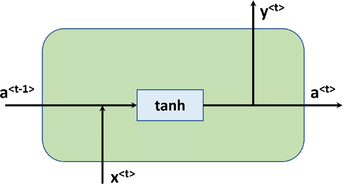
\includegraphics[width=0.23\textwidth]{RNN_cell_architecture.png}}
	\quad
	\subfloat[][]{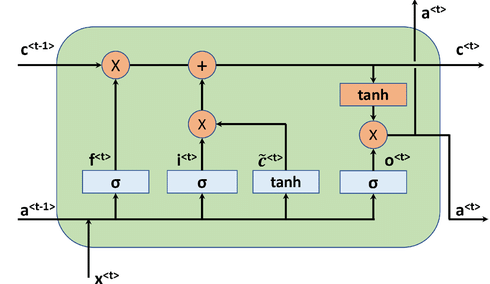
\includegraphics[width=0.23\textwidth]{LSTM_cell_architecture.png}}
	\caption{Different \gls{rnn} cell architectures: (a): Simple RNN unit, (b): LSTM unit \cite{Chen2021}}
	\label{fig:RNN-classification}
\end{figure}

However, standard \glspl{rnn} have some major drawbacks, such as the vanishing or exploding gradient problem, which limit their application \cite{Bengio1994}. \gls{lstm} networks (Hochreiter and Schmidhuber \cite{Hochreiter1997}) avoid this problem and have established themselves as one of the most used Deep Learning model type, especially for \gls{nlp} \cite{Wu2016}. For these reasons \glspl{lstm} will be one of the investigated \gls{rnn} approaches in this project. Another investigated \gls{rnn} approach is the \gls{gru}. It is a simplified version of the \gls{lstm}. Due to this simplicity it has been gaining in popularity in recent years \cite{Rana2016}. 

The key idea to \glspl{gru} and \glspl{lstm} is the memory cell which allows the network to remember information without much loss.

The \gls{lstm} architecture consists of an input gate, a forget gate and an output gate. The input gate decides to add new information from the present input to the present cell state scaled by how much it wishes to add them. The forget gate allows the cell to know how to partially forget the previous cell state. Then, the output gate decides what to output from the new cell state.

% What is the candidate?

For the \gls{gru} architecture, only two gates are implemented. The update gate decides the portion of updated candidate needed to calculate the current cell state, which in turn also decides the portion of the previous cell state retained. The relevance gate calculates how relevant the previous information is, and then is used in the candidate for the updated value.

A simple \gls{rnn} architecture will also be explored to evaluate the possible benefits of more complex architectures such as \glspl{lstm} and \glspl{gru}. A \gls{rnn} unit only has a tanh layer after combining the cell state and the candidate.

\subsection{Convolutional Neural Networks}
\label{sec:convolutional_neural_networks}

Recent results suggest that \glspl{cnn} can match or even outperform \glspl{rnn} in time series related tasks \cite{Bai2018}. The second major network type of this work are therefore \glspl{cnn}.

The common \gls{cnn} models deal with 2-Dimensional data as input such as pictures. The time sequence data used for \gls{phm} is in 1-Dimensional format. For this application 1D-\gls{cnn} have been introduced. The key differences between them and the 2D-\glspl{cnn} are that their input data is reduced by one dimension and that the convolution filter only slides in one direction \cite{Akrim2021}. Figure \ref{fig:1D_cnn_architecture} shows an example of a simple 1D-\gls{cnn} architecture with an illustration of the filter sliding over the time series. 

\begin{figure}[htp]
	\centering
	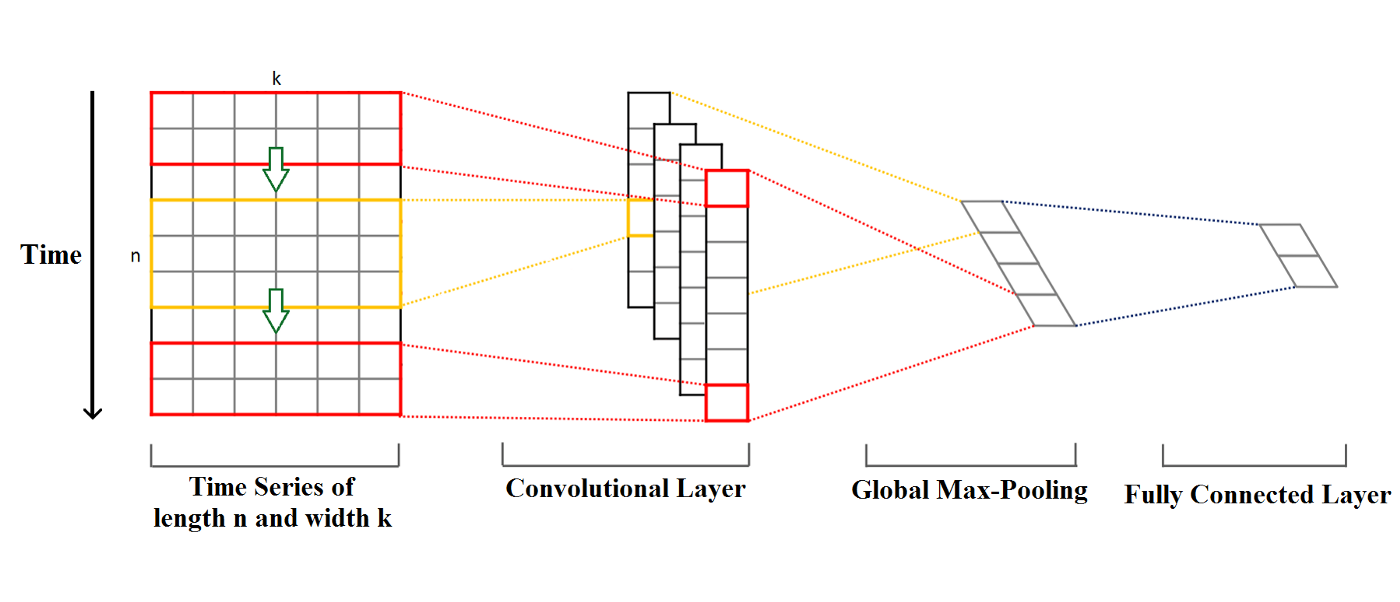
\includegraphics[width=0.45\textwidth]{1D_CNN_Architecture.png}
	\caption{Example of a 1D-\gls{cnn} architecture \cite{Sayyad}}
	\label{fig:1D_cnn_architecture}
\end{figure}

Besides the 1D-\gls{cnn} architecture \glspl{tcn} (Bai et al. \cite{Bai2018}) are investigated in this work. A \gls{tcn} is a specific \gls{cnn} architecture that tries to replicate some of the best practices for \gls{cnn} architectures. As depicted in Fig. \ref{fig:tcn_architecture} a \gls{tcn} is composed of multiple layers which include dilation. The dilation for each layer can be set arbitrarily but it is common practice to use multiples of $ 2 $ for it. Through dilation \glspl{tcn} can increase their receptive field and therefore capture relationships over longer time sequences. One \gls{tcn} layer is composed of a \gls{tcn} residual block (see Figure \ref{fig:tcn_block} (a)). One block consists of two dilated convolutional layers. The activation function for the layers is usually the ReLU function. The residual blocks include dropout and normalization layers between the convolutional layers. The blocks also include an optional skip connection with a 1x1 convolutional layer. Figure \ref{fig:tcn_block} (b) shows an exemplary \gls{tcn} block with a kernel size of $ k = 3 $ and a dilation of $ d = 1 $. For more details on \glspl{tcn} see \cite{Bai2018}.

\begin{figure}[htp]
	\centering
	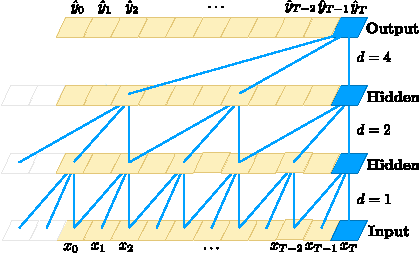
\includegraphics[width=7cm]{tcn_architecture.pdf}
	\caption{\gls{tcn} with dilation factors d = 1; 2; 4 and filter size k = 3 \cite{Bai2018}}
	\label{fig:tcn_architecture}
\end{figure}

\begin{figure}[htp]
	\centering
	\subfloat[][]{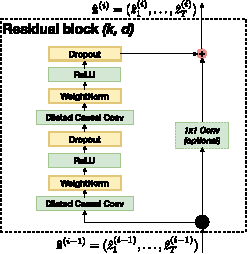
\includegraphics[width=0.23\textwidth]{tcn_block.pdf}}
	\quad
	\subfloat[][]{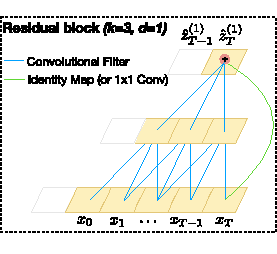
\includegraphics[width=0.23\textwidth]{tcn_block_example.pdf}}
	\caption{\gls{tcn} block elements: (a): Generic \gls{tcn} block, (b): Example for a \gls{tcn} block \cite{Bai2018}}
	\label{fig:tcn_block}
\end{figure}

\subsection{Metric and loss function}
\label{sec:metric_and_loss_function}

To evaluate the performance of developed models a metric is needed. As the networks are used to perform classification instead of regression the accuracy metric is used. This metric calculates how many of the predictions made with the used dataset are correct (e.g. the right \gls{rul} range is predicted)

\begin{equation}
	\label{eq:accuracy_metric}
	Accuracy = \frac{Number \: of \: correct \: predictions}{Total \: number \: of \: predictions}.
\end{equation}

This metric is applied during training and validation to compare different models against each other. The final assessment of the models is made by applying the accuracy metric to the testing dataset.

The used loss function which is used as the objective function for minimization by the backpropagation algorithm is the categorical crossentropy loss function

\begin{equation}
	\label{eq:categorical-cross-entrophy}
	CE = -log(\frac{e^{s_p}}{\sum_{j}^{C} e^{s_j}})	
\end{equation}

where $ s_j $ is the output of the network for Class $ j $ with $ s_p $ being the output for the positive class of the sample.

\subsection{Hyperparameter Optimization}
\label{sec:hyperparameter_optimization_method}

To optimize the proposed network architectures a hyperparameter optimization is performed. The hyperparameters include the parameters for the training process (Learning rate, batch size etc.), network parameters (Dropout rate, activation function etc.) and the network architecture itself (number of layers, size of the layers etc.).

There are different strategies for hyperparameter optimization which can be divided in Model-Free and Model-Based approaches. For this study only Model-Free approaches are considered as they are more common and easier to apply. The two typical Model-Free approaches are Grid Search and Random Search \cite{Feurer2019}. 

For Grid Search the user defines a discrete number of values for each parameter. The algorithm then tests all possible combinations of these sets of values. This quickly leads to an excessive amount of training runs that need to be done as the number of possible combinations $ B $ grows exponentially with the dimensionality $ d $ of the search space. If the number of values per parameter is $ n = 3 $ and the dimensionality is just $ d = 5 $ the number of combinations already equals $ B = n^d = 243 $.

Random Search works with a fixed number of evaluations where for each evaluation a value randomly is selected from a predefined set of values for each parameter. The set of values can either be continuous with a lower and upper bound for the values or a discrete set of values. Random Search works better than Grid Search when some parameters are more important than others, which is a property that holds true in many cases \cite{Feurer2019}. Figure \ref{fig:grid_search_random_search} illustrates this property for one important and one unimportant parameter. With a fixed amount of $ B $ evaluations Random Search can evaluate up to $ B $ different values for each parameter. Whereas Grid Search is limited to $ B^{1/N} $ values per parameter. It can be expected that the networks used in this study behave like most networks with regard to the varying importance of the hyperparameters and therefore Random Search is chosen for hyperparameter optimization.

\begin{figure}[htp]
	\centering
	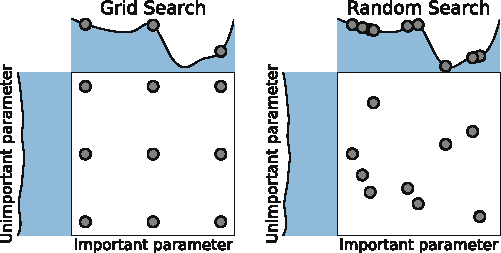
\includegraphics[width=7cm]{grid_search_random_search.pdf}
	\caption{Comparison of grid search and random search with 9 evaluations on an important and an unimportant parameter  \cite{Feurer2019}}
	\label{fig:grid_search_random_search}
\end{figure}

To select the best model after performing the hyperparameter optimization the accuracy of the model on the validation dataset is used.

\subsection{Fine Tuning}
\label{sec:fine_tuning}

After the optimum parameters for a model are found the model can be further improved by running more training epochs. To do so the models are trained with \gls{lrdecay}. This approach decreases the learning rate incrementally after a certain number of epochs.
In this case the best models from the hyperparameter optimization are taken and trained for a predefined number of epochs on the learning rate which was identified as the best one in the hyperparameter optimization. The learning rate is then lowered before the model is trained again for a fixed number of epochs. This step is repeated until convergence is achieved and no more significant improvements are visible. By using this approach the model in the early stages of training is less likely to get stuck in a local minimum and explores a wider range of possible configurations. As the training comes closer to an optimum the decaying learning rate helps with convergence and avoiding oscillations. According to You et al. \cite{You2019} there are probably more reasons to the effectiveness of \gls{lrdecay} besides this common beliefs. The initially large learning rate is, according to them, preventing the network from memorizing noisy data while the decaying learning rate helps with learning complex patterns in the dataset in the later stages of training.

\section{Results}
\label{sec:results}

\subsection{Model architectures}
\label{sec:model_architectures}

All \gls{rnn} architectures are based on the same template. The dataset being normalized before being fed to the models, there is no need for a specific normalization layer. A flexible number of layers is implemented in the networks, as well as a flexible number of cells in each layer which is always a power of $ 2 $. A possible dropout and recurrent dropout can also be added to each layer. At the end of the architecture, a dense layer with $ 20 $ units is added in order to match the number of \gls{rul} classes $ C = 20 $.  

Based on the \gls{cnn} architecture of Li et al. \cite{Li2018} which was used for aero-engine \gls{rul} prediction a 1D-\gls{cnn} architecture is generated. The first layer of the architecture is for layer normalization. Afterwards a flexible number of 1D-convolutional layers are added which all have the same number of filters and an identical kernel size. The output of the convolutional layers is flattend before being fed into the final dense output layer which has $ 20 $ nodes to match the number of \gls{rul} classes $ C = 20 $. As an example Figure \ref{fig:cnn_architecture_1000_structures} shows the final architecture after the hyperparameter optimization with $ 1000 $ training structures.

\begin{figure}[htp]
	\centering
	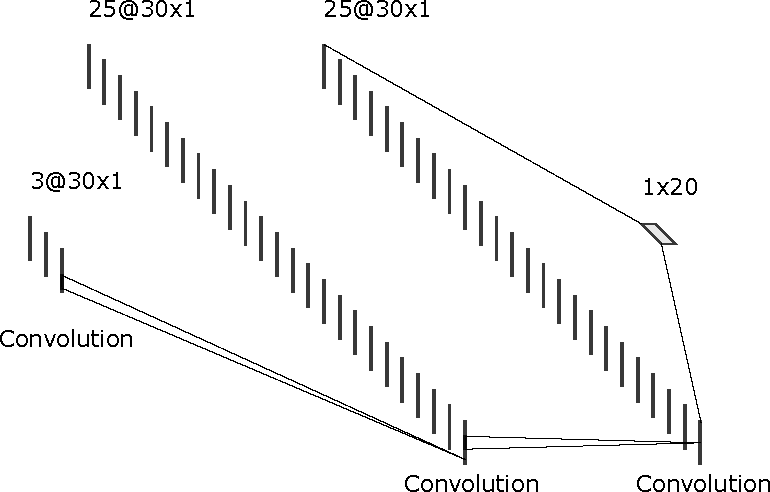
\includegraphics[width=0.45\textwidth]{cnn_architecture_1000_structures.pdf}
	\caption{1D-\gls{cnn} architecture after hyperparameter optimization with 1000 training structures}
	\label{fig:cnn_architecture_1000_structures}
\end{figure}

A \gls{tcn} architecture template is generated based on the results of Liu et al. \cite{Liu2019} who used the network for \gls{rul} prediction of roller bearings. The architecture consists of multiple \gls{tcn} residual blocks with the dilation increasing with multiples of $ 2 $ for each additional layer. The first layer has a dilation of $ d = 1 $. Each \gls{tcn} block features the same number of filters with an identical kernel size. The layer after the \gls{tcn} blocks is the dense output layer which has $ 20 $ nodes to match the number of \gls{rul} classes $ C = 20 $. The skip connection layer is activated for all \gls{tcn} residual blocks.

\subsection{Hyperparameter optimization}
\label{sec:hyperparameter_optimization_results}

The hyperparameter optimization is performed using Random Search as described in section \ref{sec:methods}. The used training dataset consists of $ 100 $, $ 500 $ or $ 1000 $ structures. For validation always the same $ 100 $ structures different to the training structures are used. The model selection after the optimization is based on the accuracy of the models on the validation dataset. Not all available parameters of the networks are considered for the optimization as that would increase the computational effort drastically. The reduction also helps to shift the focus of the optimization on the important parameters and avoid varying parameters which have no or only little influence on the accuracy of the network.

\subsubsection{\gls{rnn}, \gls{lstm} and \gls{gru} hyperparameter optimization}
\label{sec:rnn_hyperparameter_optimization}

Following the same method used for the 1D-\gls{cnn} and \gls{tcn} hyperparameter optimization, fixed parameters are set for each architecture, to avoid searching for hyperparameters which are not relevant to the accuracy improvement. Those fixed parameters are the same for the \gls{rnn}, \gls{lstm} and \gls{gru} architectures, and can be found in Table \ref{tab:fixed_parameters_rnn_optimization}.

\begin{table}[htp]
	\centering
	\caption{Fixed parameters for \gls{rnn}, \gls{lstm} and \gls{gru} hyperparameter optimization}
	\label{tab:fixed_parameters_rnn_optimization}
	\begin{tabular}{ll}
		\textbf{Parameter} & \textbf{Value} \\
		\hline
		Batch size & $ 4096 $ \\
		Activation function & ReLU \\
		Epochs & $ 500 $ \\
		Sequence length & $ 30 $ 
	\end{tabular}
\end{table}

Once those parameters are fixed, useful hyperparameters are identified. These are the ones which can have a significant impact on accuracy improvement. They were identified on $ 100 $ structures, and then reused for $ 500 $ structures. The optimization on $ 1000 $ structures was not done due to a lack of time. The resulting model of the optimization on $ 500 $ structures was later used in section \ref{sec:rnn_fine_tuning_results} for the fine tuning on $ 1000 $ structures. The found variable hyperparameters are the same for the \gls{rnn}, \gls{lstm} and \gls{gru} models. They can be found in Table \ref{tab:variable_parameters_rnn_optimization}.

\begin{table}[htp]
	\centering
	\caption{Variable parameters for \gls{rnn}, \gls{lstm} and \gls{gru} hyperparameter optimization}
	\label{tab:variable_parameters_rnn_optimization}
	\begin{tabular}{ll}
		\textbf{Parameter} & \textbf{Value set} \\
		\hline
		Number of hidden layers & $ \{1, 2, 3\} $ \\
		Number of cells per layer & $ \{32, 64, 128, 256\} $ \\
		Dropout rate & $ \{0, 0.1\} $ \\
		Recurrent Dropout rate & $ \{0, 0.1\} $ \\
		Learning rate & $ \{10^{-2}, 10^{-3}\} $
	\end{tabular}
\end{table}

The Random Search strategy was then used to optimize those hyperparameters on $ 100 $ and $ 500 $ structures, with a fixed sliding window size of $ 30 $. The learning rate is not listed in the results as the fine tuning will use an adaptative learning rate strategy to optimize the performance of the network. The results of the hyperparameter optimization of the \glspl{rnn}, \glspl{lstm} and \glspl{gru} can be found in Table \ref{tab:results_parameters_rnn_optimization}.

\begin{table}[htp]
	\centering
	\caption{Best models of the \gls{rnn}, \gls{lstm} and \gls{gru} hyperparameter optimization for $ 100 $ and $ 500 $ training structures}
	\label{tab:results_parameters_rnn_optimization}
	\setlength{\tabcolsep}{3pt} % Default value: 6pt
	\begin{tabular}{p{2.5cm}|lll|lll}
		Training structures & \multicolumn{3}{c}{$ 100 $} & \multicolumn{3}{c}{$ 500 $} \\
		\hline
		Type of architecture & \gls{rnn} & \gls{lstm} & \gls{gru} & \gls{rnn} & \gls{lstm} & \gls{gru}\\
		\hline
		Number of hidden layers & $3$ & $2$ & $3$ & $3$ & $2$ & $2$ \\
		Number of cells per layer & $32$ & $64$ & $256$ & $32$ & $128$ & $256$ \\
		Dropout rate & $0$ & $0$ & $0$ & $0$ & $0$ & $0$ \\
		Recurrent Dropout rate & $0$ & $0$ & $0$& $0$ & $0$ & $0$ \\
		\hline
		Validation accuracy & $0.752$ & $0.688$ & $0.726$ & $0.871$ & $0.700$ & $0.814$
	\end{tabular}
\end{table}

The results show that \glspl{rnn} do not need many layers to get a good accuracy compared to \glspl{cnn}. The best accuracy can be found with no more than $ 2 $ or $ 3 $ layers in this case. Indeed, too many layers and cells for this amount of data might lead to the model loosing itself, along with the fact that the computational time increases drastically. The Dropout and Recurrent Dropout rates were optimal at $ 0 \% $ meaning that the models did not overfit without dropout for this set of structures. This conclusion is supported by the training history of the model fine tuning shown in Figures \ref{fig:accuracy_100_structures_fine_tuning_rnn}, \ref{fig:accuracy_500_structures_fine_tuning_rnn} and \ref{fig:accuracy_1000_structures_fine_tuning_rnn} where the validation accuracy follows the training accuracy.

\subsubsection{1D-\gls{cnn} and \gls{tcn} hyperparameter optimization}
\label{sec:cnn_hyperparameter_optimization}

Table \ref{tab:fixed_parameters_cnn_optimization} lists the fixed parameters of the 1D-\gls{cnn} optimization. The sliding window length includes multiple values as the influence of that parameter is studied by performing multiple optimization runs with different lengths of the sliding window.

\begin{table}[htp]
	\centering
	\caption{Fixed parameters for 1D-\gls{cnn} hyperparameter optimization}
	\label{tab:fixed_parameters_cnn_optimization}
	\begin{tabular}{ll}
		\textbf{Parameter} & \textbf{Value} \\
		\hline
		Batch size & $ 4096 $ \\
		Sliding window length & $ \{5, 10, 15, 20, 30, 40\} $ \\
		Activation function & ReLU \\
		Padding & Padding with zeros \\
		Dropout & No dropout
	\end{tabular}
\end{table}

Table \ref{tab:variable_parameters_cnn_optimization} lists the variable parameters and their set of possible values for the \gls{cnn} hyperparameter optimization. The chosen range for the parameters is the result of a preliminary analysis to identify meaningful boundaries for them.

\begin{table}[htp]
	\centering
	\caption{Variable parameters for 1D-\gls{cnn} hyperparameter optimization}
	\label{tab:variable_parameters_cnn_optimization}
	\begin{tabular}{ll}
		\textbf{Parameter} & \textbf{Value set} \\
		\hline
		Number of convolutional layers & $ \{2, 4, 6, 8\} $ \\
		Number of filters per layer & $ \{15, 20, 25, 30, 35, 40, 45, 50\} $ \\
		Kernel size & $ \{3, 6, 9, 12\} $ \\
		Learning rate & $ \{10^{-2}, 10^{-3}\} $
	\end{tabular}
\end{table}

For the 1D-\gls{cnn} the hyperparameter optimization is performed on $ 100 $, $ 500 $ and $ 1000 $  training structures. For the smallest dataset of $ 100 $ structures the optimization is performed on the full range of different sliding window lengths as listed in Table \ref{tab:variable_parameters_cnn_optimization}. The optimizations on $ 500 $ and $ 1000 $ structures are only performed with a sliding window size of $ N = 30 $. All optimization runs are performed with $ B = 100 $ evaluations for $ 500 $ training epochs each.

Figure \ref{fig:influence_sequence_length_cnn} shows the achieved maximum validation accuracy after the hyperparameter optimization for different lengths of the sliding window. The accuracy increases approximately linearly with size of the sliding window although the absolute value of the improvement remains relatively small. The size of the sliding window can not be increased much above a size of $ 40 $ as then the sliding window would be larger than the time series of some of the structures. A too big sliding window besides that has the disadvantage that it can only be applied if enough data to fill the sliding window is already collected. This means that there could be situations in which the first predictions can only be made just before the part fails or in the worst case after it failed. As a result of these considerations and because of the negligible difference between the sliding window sizes of $ 30 $ and $ 40 $ a size of $ N = 30 $ is chosen for all further hyperparameter optimization runs with the 1D-\gls{cnn} on $ 500 $ and $ 1000 $ structures.

\begin{figure}[htp]
	\centering
	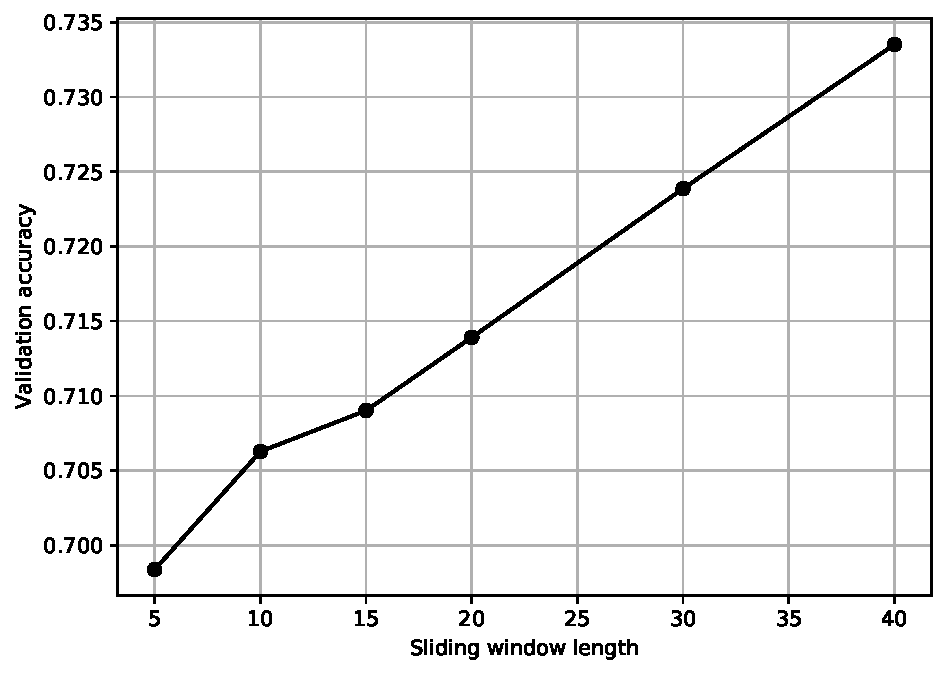
\includegraphics[width=0.35\textwidth]{python/influence_sequence_length_cnn.pdf}
	\caption{1D-\gls{cnn} hyperparameter optimization for different sliding window sizes for training on $ 100 $ structures}
	\label{fig:influence_sequence_length_cnn}
\end{figure}

Table \ref{tab:hyperparameters_100_structures_cnn} shows the different architectures from the hyperparameter optimizations that achieved the best results with the respective sliding window length on $ 100 $ training structures. There is no clear trend for the network architecture in relation to the sliding window size. This is backed by the fact that the 2nd and 3rd best networks for each respective hyperparameter optimization can also have significantly different architectures to the best one. This observation leads to the conclusion that there are many different network architectures that can give equal results.

\begin{table}[htp]
	\centering
	\caption{Best models of the 1D-\gls{cnn} hyperparameter optimization on $ 100 $ structures for different sliding window lengths}
	\label{tab:hyperparameters_100_structures_cnn}
	\setlength{\tabcolsep}{3pt} % Default value: 6pt
	\begin{tabular}{p{2.5cm}|llllll}
		Sliding window size & $ 5 $ & $ 10 $ & $ 15 $ & $ 20 $ & $ 30 $ & $ 40 $ \\
		\hline
		Number of convolutional layers & $ 4 $ & $ 2 $ & $ 4 $ & $ 2 $ & $ 6 $ & $ 6 $ \\
		Number of filters per layer & $ 25 $ & $ 35 $ & $ 30 $ & $ 45 $ & $ 20 $ & $ 20 $ \\
		Kernel size & $ 3 $ & $ 6 $ & $ 9 $ & $ 9 $ & $ 6 $ & $ 3 $ \\
		Learning rate & $ 10^{-2} $ & $ 10^{-2} $ & $ 10^{-2} $ & $ 10^{-2} $ & $ 10^{-2} $ & $ 10^{-2} $ \\
		\hline
		Validation accuracy & $ 0.698 $ & $ 0.706 $ & $ 0.709 $ & $ 0.714 $ & $ 0.724 $ & $ 0.734 $
	\end{tabular}
\end{table}

Figure \ref{fig:accuracy_100_structures_random_search_cnn} shows the history of the training and validation accuracy for the training on $ 100 $ structures for some of the different sliding window sizes. There is little to no overfitting on the training dataset for all of the training runs. The $ 500 $ training epochs lead to a sufficient convergence of all the runs.

\begin{figure}[htp]
	\centering
	\subfloat[][]{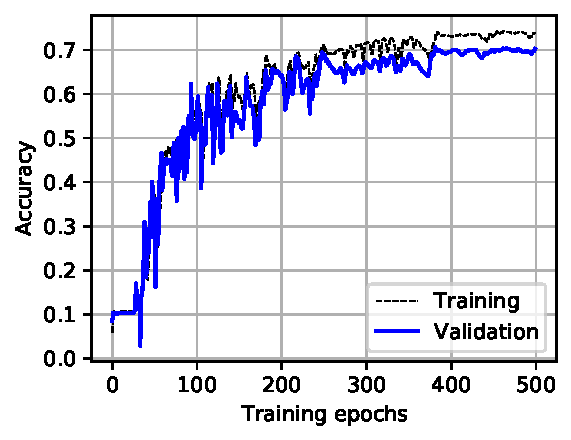
\includegraphics[width=0.23\textwidth]{python/accuracy_100_structures_random_search_10_CNN.pdf}}
	\quad
	\subfloat[][]{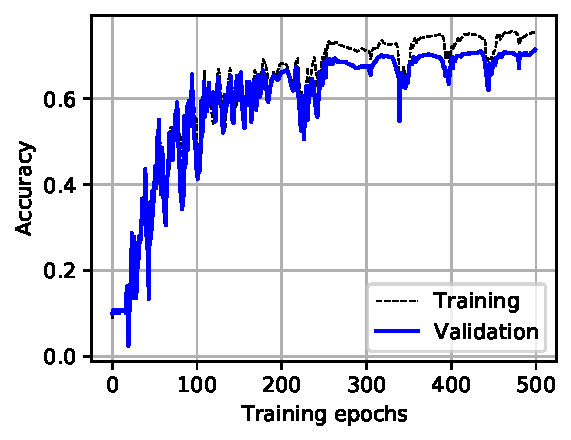
\includegraphics[width=0.23\textwidth]{python/accuracy_100_structures_random_search_20_CNN.pdf}}
	\\
	\subfloat[][]{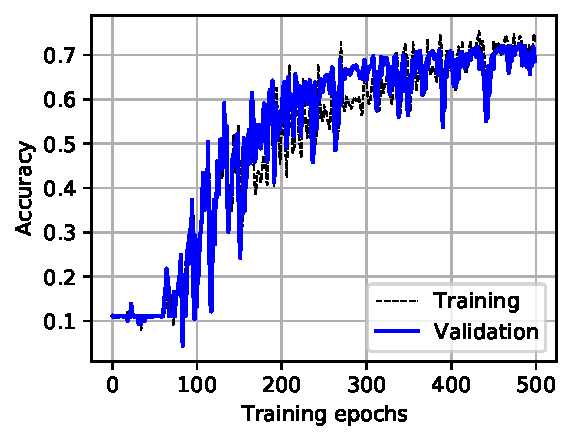
\includegraphics[width=0.23\textwidth]{python/accuracy_100_structures_random_search_30_CNN.pdf}}
	\quad
	\subfloat[][]{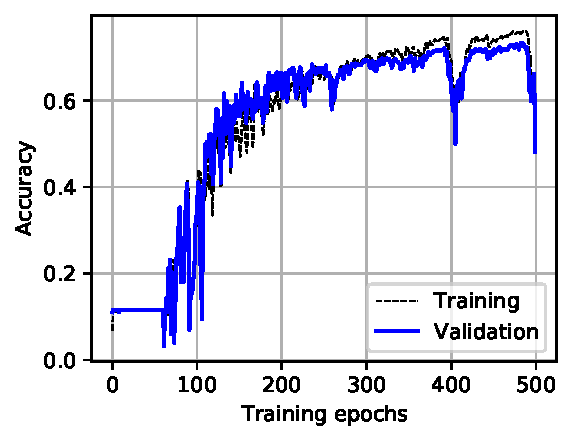
\includegraphics[width=0.23\textwidth]{python/accuracy_100_structures_random_search_40_CNN.pdf}}
	\caption{Training and validation accuracy history for the best models of the 1D-\gls{cnn} hyperparameter optimization on $ 100 $ training structures with a sliding window size of: (a): $ 10 $, (b): $ 20 $, (c): $ 30 $, (d): $ 40 $}
	\label{fig:accuracy_100_structures_random_search_cnn}
\end{figure}

The hyperparameter optimization of the 1D-\gls{cnn} with $ 500 $ training structures and a sliding window size of $ 30 $ leads to an improvement of the validation accuracy. Showing that the network architecture if provided with more data can better learn the relationships within the dataset. An increase of the training dataset to $ 1000 $ structures leads to no further improvement. This is the result of the lower learning rate of this network which has not fully converged yet (see Figure \ref{fig:accuracy_500_1000_structures_random_search_CNN})  Table \ref{tab:hyperparameters_100_500_1000_structures_CNN} depicts the best network architectures together with the achieved validation accuracy for $ 100 $, $ 500 $ and $ 1000 $ training structures with a sliding window size of $ 30 $. There is not clear trend visible in the network architectures indicating that there are many different architectures possible which achieve similar results. This hypothesis is supported by the similar results achieved by some of the other architectures created by the hyperparameter optimizations with distinctly different architectures.

\begin{table}[htp]
	\centering
	\caption{Best models of the 1D-\gls{cnn} hyperparameter optimization for $ 100 $, $ 500 $ and $ 1000 $ training structures}
	\label{tab:hyperparameters_100_500_1000_structures_CNN}
	\begin{tabular}{p{2.5cm}|llllll}
		Training structures & $ 100 $ & $ 500 $ & $ 1000 $ \\
		\hline
		Sliding window size & \multicolumn{3}{c}{$ 30 $} \\
		\hline
		Number of convolutional layers & $ 6 $ & $ 2 $ & $ 4 $ \\
		Number of filters per layer & $ 20 $ & $ 40 $ & $ 25 $ \\
		Kernel size & $ 6 $ & $ 12 $ & $ 9 $ \\
		Learning rate & $ 10^{-2} $ & $ 10^{-2} $ & $ 10^{-3} $ \\
		\hline
		Validation accuracy & $ 0.724 $ & $ 0.788 $ & $ 0.789 $
	\end{tabular}
\end{table}

Figure \ref{fig:accuracy_500_1000_structures_random_search_CNN} shows the training history of the best models of the 1D-\gls{cnn} hyperparameter optimization when training with $ 500 $ and $ 1000 $ structures respectively. None of the two models shows significant overfitting on the training dataset. Both models are not yet fully converged and therefore have room for improvement. This potential is exploited in the model fine tuning in section \ref{sec:cnn_fine_tuning_results}. The training history of the model trained on $ 500 $ structures shows an instability at around $ 480 $ epochs. Indicating that the learning rate should be reduced which is done in the subsequent model fine tuning.

\begin{figure}[htp]
	\centering
	\subfloat[][]{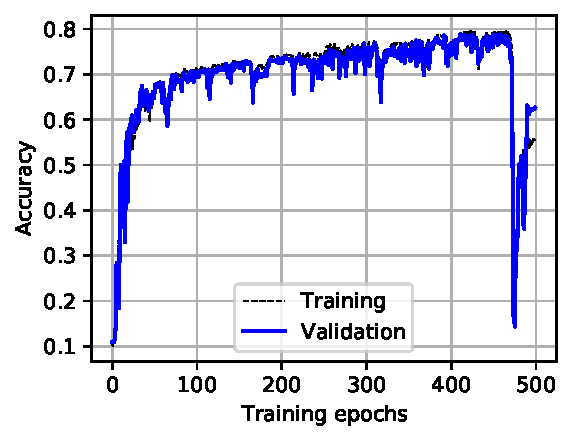
\includegraphics[width=0.23\textwidth]{python/accuracy_500_structures_random_search_CNN.pdf}}
	\quad
	\subfloat[][]{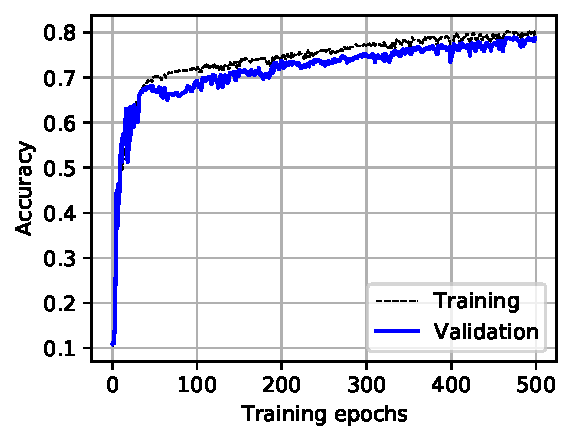
\includegraphics[width=0.23\textwidth]{python/accuracy_1000_structures_random_search_CNN.pdf}}
	\caption{Training and validation accuracy history for the best models of the 1D-\gls{cnn} hyperparameter optimization on (a): $ 500 $ and (b): $ 1000 $ training structures}
	\label{fig:accuracy_500_1000_structures_random_search_CNN}
\end{figure}

Table \ref{tab:fixed_parameters_tcn_optimization} lists the fixed parameters of the \gls{tcn} hyperparameter optimization. The sliding window length includes multiple values as the influence of that parameter is studied by performing multiple optimization runs with different lengths of the sliding window.

\begin{table}[htp]
	\centering
	\caption{Fixed parameters for \gls{tcn} hyperparameter optimization}
	\label{tab:fixed_parameters_tcn_optimization}
	\begin{tabular}{ll}
		\textbf{Parameter} & \textbf{Value} \\
		\hline
		Batch size & $ 4096 $ \\
		Sliding window length & $ \{10, 15, 20, 30\} $ \\
		Activation function & ReLU \\
		Padding & Causal padding \\
		Normalization & Weight normalization
	\end{tabular}
\end{table}

Table \ref{tab:variable_parameters_tcn_optimization} lists the variable parameters and their set of possible values for the \gls{tcn} hyperparameter optimization. The chosen range for the parameters is the result of a preliminary analysis to identify meaningful boundaries for them. The indicated number of layers directly corresponds the maximal dilation as the dilations rises with multiples of two for each \gls{tcn} block. For e.g. $ 4 $ blocks the dilation in the blocks is $ [1, 2, 4, 8] $.

\begin{table}[htp]
	\centering
	\caption{Variable parameters for \gls{tcn} hyperparameter optimization}
	\label{tab:variable_parameters_tcn_optimization}
	\begin{tabular}{ll}
		\textbf{Parameter} & \textbf{Value set} \\
		\hline
		Number of layers & $ \{4, 6, 8, 10\} $ \\
		Number of filters per layer & $ \{15, 20, 25, 30, 35, 40, 45, 50\} $ \\
		Kernel size & $ \{3, 6, 9, 12\} $ \\
		Dropout rate & $ \{0.0, 0.1, 0.2\} $ \\
		Learning rate & $ \{10^{-2}, 10^{-3}\} $
	\end{tabular}
\end{table}

As for the 1D-\gls{cnn} the hyperparameter optimization for the \gls{tcn} is performed on $ 100 $, $ 500 $ and $ 1000 $  training structures. For the smallest dataset of $ 100 $ structures the optimization is performed on the full range of different sliding window lengths as listed in Table \ref{tab:variable_parameters_tcn_optimization}. The optimizations on $ 500 $ and $ 1000 $ structures are only performed with a sliding window size of $ N = 30 $. All optimization runs are performed with $ B = 50 $ evaluations for $ 500 $ training epochs each. The number of evaluations is reduced compared to the \gls{cnn} optimization because of the increased computational effort for the \glspl{tcn}.

Figure \ref{fig:influence_sequence_length_tcn} shows the achieved maximum validation accuracy after the hyperparameter optimization for different lengths of the sliding window. There is a significant increase of the accuracy between a length of $ 15 $ and $ 30 $. The other variations seem to be the result of scatter as a consequence of neural network training in general as well as the Random Search which leads to different network architectures in each optimization run. To keep a big enough distance to the drop in accuarcy for windows sizes $ \leq 20 $ a sliding window size of $ N = 30 $ is chosen for all further hyperparameter optimizations with the \gls{tcn} on $ 500 $ and $ 1000 $ structures.

\begin{figure}[htp]
	\centering
	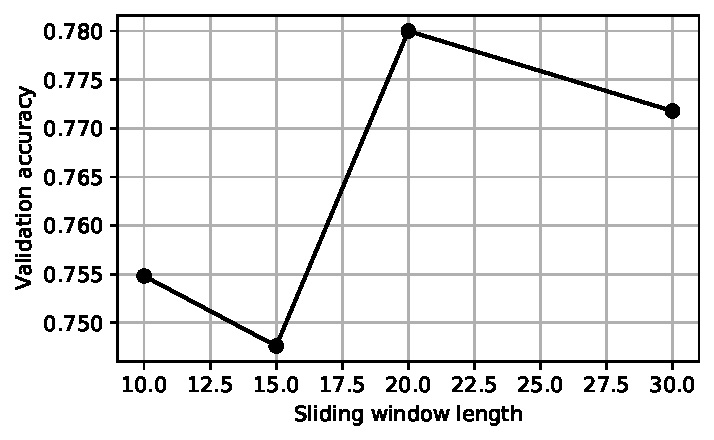
\includegraphics[width=0.35\textwidth]{python/influence_sequence_length_tcn.pdf}
	\caption{\gls{tcn} hyperparameter optimization for different sliding window sizes for training on $ 100 $ structures}
	\label{fig:influence_sequence_length_tcn}
\end{figure}

Table \ref{tab:hyperparameters_100_structures_tcn} shows the different architectures from the hyperparameter optimizations that achieved the best results with the respective sliding window length on $ 100 $ training structures. There is a clear trend for the network architecture to have $ 6 $ or $ 8 $ \gls{tcn} residual blocks, a kernel size of $ 2 $ and no dropout.

\begin{table}[htp]
	\centering
	\caption{Best models of the \gls{tcn} hyperparameter optimization on $ 100 $ structures for different sliding window lengths}
	\label{tab:hyperparameters_100_structures_tcn}
	%\setlength{\tabcolsep}{3pt} % Default value: 6pt
	\begin{tabular}{p{2.5cm}|llllll}
		Sliding window size & $ 10 $ & $ 15 $ & $ 20 $ & $ 30 $ \\
		\hline
		Number of \gls{tcn} residual blocks & $ 6 $ & $ 8 $ & $ 8 $ & $ 8 $ \\
		Number of filters per layer & $ 30 $ & $ 45 $ & $ 25 $ & $ 30 $ \\
		Kernel size & $ 2 $ & $ 2 $ & $ 2 $ & $ 2 $ \\
		Dropout rate & $ 0.0 $ & $ 0.0 $ & $ 0.0 $ & $ 0.0 $ \\
		Learning rate & $ 10^{-2} $ & $ 10^{-2} $ & $ 10^{-2} $ & $ 10^{-3} $ \\
		\hline
		Validation accuracy & $ 0.755 $ & $ 0.748 $ & $ 0.780 $ & $ 0.771 $
	\end{tabular}
\end{table}

Figure \ref{fig:accuracy_100_structures_random_search_cnn} shows the history of the training and validation accuracy for different sliding window sizes for the training with $ 100 $ structures. There is little to no overfitting on the training dataset for all of the training runs. The $ 500 $ training epochs lead to a sufficient convergence of all the runs.

\begin{figure}[htp]
	\centering
	\subfloat[][]{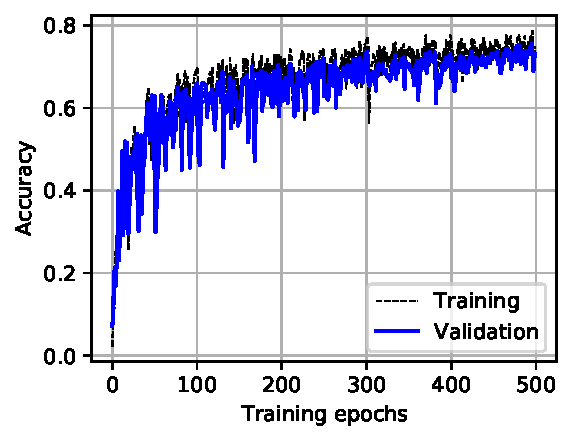
\includegraphics[width=0.23\textwidth]{python/accuracy_100_structures_random_search_10_TCN.pdf}}
	\quad
	\subfloat[][]{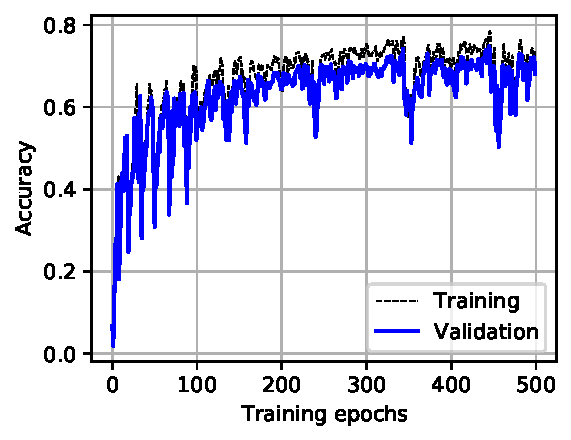
\includegraphics[width=0.23\textwidth]{python/accuracy_100_structures_random_search_15_TCN.pdf}}
	\\
	\subfloat[][]{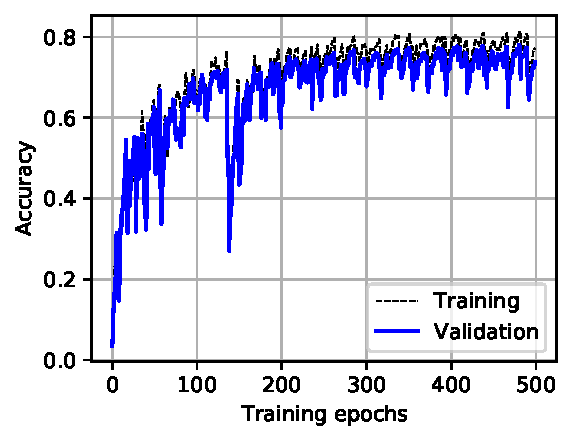
\includegraphics[width=0.23\textwidth]{python/accuracy_100_structures_random_search_20_TCN.pdf}}
	\quad
	\subfloat[][]{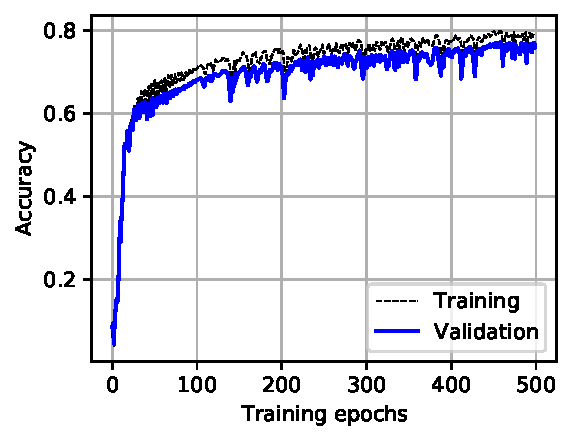
\includegraphics[width=0.23\textwidth]{python/accuracy_100_structures_random_search_30_TCN.pdf}}
	\caption{Training and validation accuracy history for the best model of the \gls{tcn} hyperparameter optimization on $ 100 $ training structures with a sliding window size of: (a): $ 10 $, (b): $ 15 $, (c): $ 20 $, (d): $ 30 $}
	\label{fig:accuracy_100_structures_random_search_tcn}
\end{figure}

Performing the hyperparameter optimization of the \gls{tcn} with $ 500 $ and $ 1000 $ structures respectively leads to significant improvements of the validation accuracy. This indicates that the network is able to better learn the relations in the dataset when feed with more data. Table \ref{tab:hyperparameters_100_500_1000_structures_TCN} depicts the best network architecture together with the achieved validation accuracy for $ 100 $, $ 500 $ and $ 1000 $ training structures with a sliding window size of $ 30 $. The resulting architectures are very similar to those depicted in Table \ref{tab:hyperparameters_100_structures_tcn} from the hyperparameter optimization performed on $ 100 $ structures with different sliding window sizes. Again featuring $ 8 $ \gls{tcn} residual blocks, a kernel size of $ 2 $ and no dropout. Indicating that there is a convergence to an optimal model architecture independent of the used training dataset.

\begin{table}[htp]
	\centering
	\caption{Best models of the \gls{tcn} hyperparameter optimization for $ 100 $, $ 500 $ and $ 1000 $ training structures}
	\label{tab:hyperparameters_100_500_1000_structures_TCN}
	\begin{tabular}{p{2.5cm}|llllll}
		Training structures & $ 100 $ & $ 500 $ & $ 1000 $ \\
		\hline
		Sliding window size & \multicolumn{3}{c}{$ 30 $} \\
		\hline
		Number of \gls{tcn} residual blocks & $ 8 $ & $ 8 $ & $ 8 $ \\
		Number of filters per layer & $ 30 $ & $ 25 $ & $ 35 $ \\
		Kernel size & $ 2 $ & $ 2 $ & $ 2 $ \\
		Dropout rate & $ 0.0 $ & $ 0.0 $ & $ 0.0 $ \\
		Learning rate & $ 10^{-3} $ & $ 10^{-2} $ & $ 10^{-2} $ \\
		\hline
		Validation accuracy & $ 0.772 $ & $ 0.883 $ & $ 0.908 $
	\end{tabular}
\end{table}

Figure \ref{fig:accuracy_500_1000_structures_random_search_TCN} shows the training history of the best models of the \gls{tcn} hyperparameter optimization when training with $ 500 $ and $ 1000 $ structures respectively. None of the two models shows a sign of overfitting on the training dataset. Both models are not yet fully converged and therefore have room for improvement. This potential is exploited in the model fine tuning in section \ref{sec:tcn_fine_tuning_results}. Both training histories show instabilities during draining, indicating that the learning rate should be reduced which is done in the subsequent model fine tuning.

\begin{figure}[htp]
	\centering
	\subfloat[][]{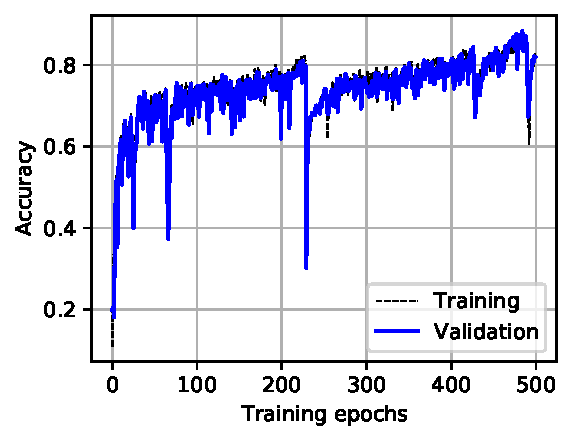
\includegraphics[width=0.23\textwidth]{python/accuracy_500_structures_random_search_TCN.pdf}}
	\quad
	\subfloat[][]{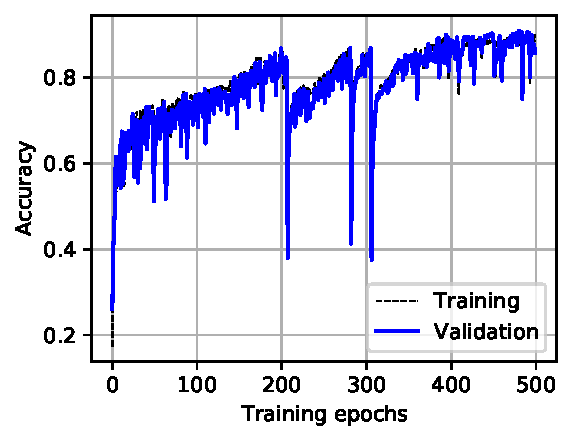
\includegraphics[width=0.23\textwidth]{python/accuracy_1000_structures_random_search_TCN.pdf}}
	\caption{Training and validation accuracy history for the best models of the \gls{tcn} hyperparameter optimization on (a): $ 500 $ and (b): $ 1000 $ training structures}
	\label{fig:accuracy_500_1000_structures_random_search_TCN}
\end{figure}

\subsection{Fine Tuning}
\label{sec:fine_tuning_results}

As the hyperparameters are optimized, the resulting models are trained with an adaptative learning rate (\gls{lrdecay}) to optimize their performance. The models are further refined on the same dataset on which the optimization was performed. \gls{lrdecay} starts with a learning rate of $10^{-2}$ or $10^{-3}$ depending on which value was chosen in the hyperparameter optimization, decreasing to $10^{-3}$, $10^{-4}$ and then $10^{-5}$. With each learning rate, the models were trained for $ 500 $ epochs which leads to maximum of $ 2000 $ training epochs. After the fine tuning the models are tested on the testing dataset to evaluate their final performance.

\subsubsection{\gls{rnn}, \gls{lstm} and \gls{gru} fine tuning}
\label{sec:rnn_fine_tuning_results}

For the \gls{rnn}, \gls{lstm} and \gls{gru} models the results of the training history can be found grouped by the number of structures in Figures \ref{fig:accuracy_100_structures_fine_tuning_rnn}, \ref{fig:accuracy_500_structures_fine_tuning_rnn} and \ref{fig:accuracy_1000_structures_fine_tuning_rnn}. It can be clearly observed that the \gls{lrdecay} strategy allows a better training for each model. Once the models are trained, they are evaluated on the testing dataset. All the results for the validation and testing accuracy can be found in Table \ref{tab:accuracy_testing_rnn_cnn}.  

\begin{figure}[htp]
	\centering
	\subfloat[][]{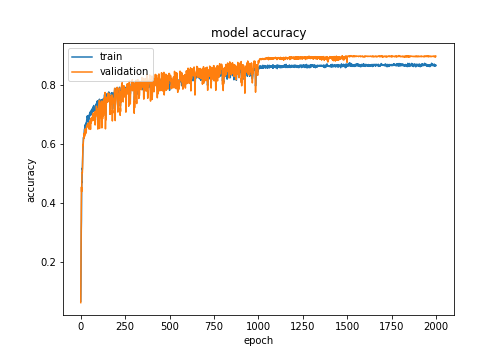
\includegraphics[width=0.23\textwidth]{fine_tuning/RNN_100_tuned_acc.png}}
	\quad
	\subfloat[][]{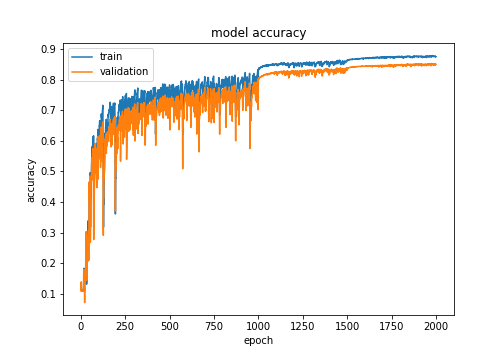
\includegraphics[width=0.23\textwidth]{fine_tuning/LSTM_100_tuned_acc.png}}
	\\
	\subfloat[][]{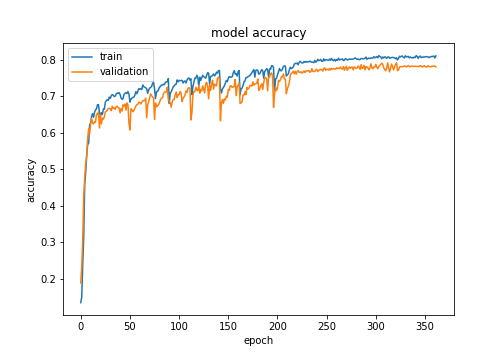
\includegraphics[width=0.23\textwidth]{fine_tuning/GRU_100_tuned_acc.png}}
	\caption{Training and validation accuracy history for $ 100 $ training structures with \gls{lrdecay}: (a): \gls{rnn}, (b): \gls{lstm}, (c): \gls{gru}}
	\label{fig:accuracy_100_structures_fine_tuning_rnn}
\end{figure}

\begin{figure}[htp]
	\centering
	\subfloat[][]{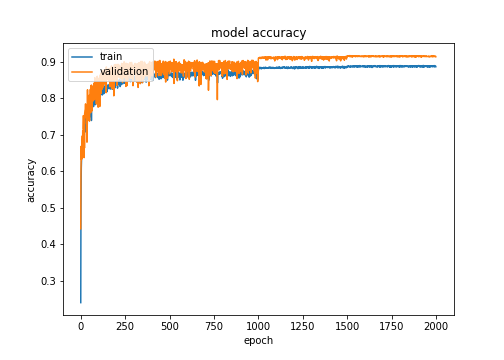
\includegraphics[width=0.23\textwidth]{fine_tuning/RNN_500_tuned_acc.png}}
	\quad
	\subfloat[][]{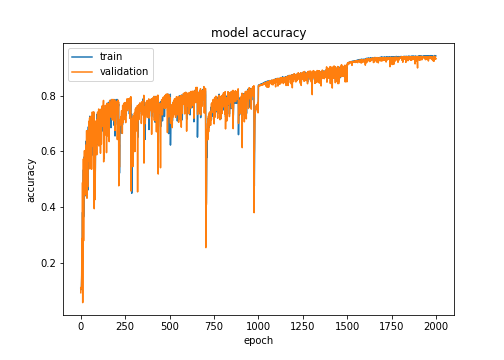
\includegraphics[width=0.23\textwidth]{fine_tuning/LSTM_500_tuned_acc.png}}
	\\
	\subfloat[][]{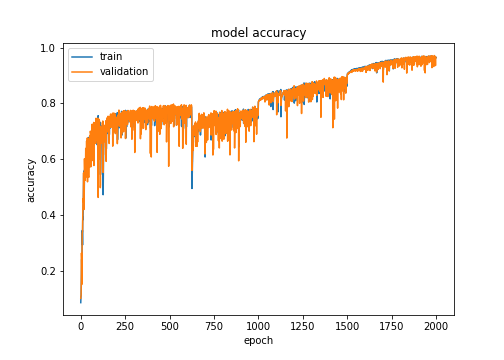
\includegraphics[width=0.23\textwidth]{fine_tuning/GRU_500_tuned_acc.png}}
	\caption{Training and validation accuracy history for $ 500 $ training structures with \gls{lrdecay}: (a): \gls{rnn}, (b): \gls{lstm}, (c): \gls{gru}}
	\label{fig:accuracy_500_structures_fine_tuning_rnn}
\end{figure}

\begin{figure}[htp]
	\centering
	\subfloat[][]{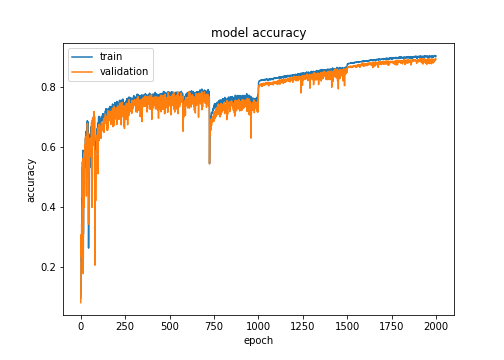
\includegraphics[width=0.23\textwidth]{fine_tuning/RNN_1000_tuned_acc.png}}
	\quad
	\subfloat[][]{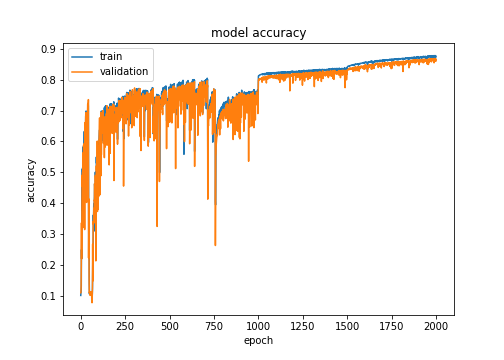
\includegraphics[width=0.23\textwidth]{fine_tuning/LSTM_1000_tuned_acc.png}}
	\\
	\subfloat[][]{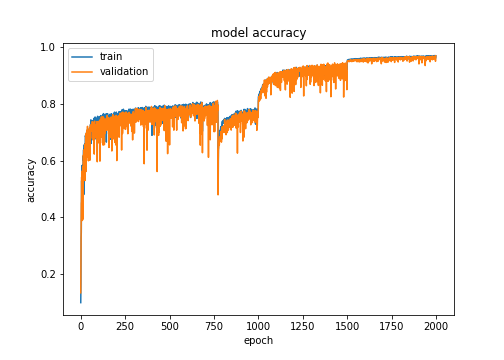
\includegraphics[width=0.23\textwidth]{fine_tuning/GRU_1000_tuned_acc.png}}
	\caption{Training and validation accuracy history for $ 1000 $ training structures with \gls{lrdecay}: (a): \gls{rnn}, (b): \gls{lstm}, (c): \gls{gru}}
	\label{fig:accuracy_1000_structures_fine_tuning_rnn}
\end{figure}

Little to no overfitting can be observed in each training. In addition, some training historys show an unstable improvement, with even a decreasing accuracy after some learning rate changes. This could have an impact on the final accuracy. Nevertheless, it seems that decreasing the learning rate improves the stability of the training.

Regarding the final validation and testing accuracies, there is a significant difference between $ 100 $ and $ 500 $ training structures. The different models increased both their validation and testing accuracies, even though the differences between $ 500 $ and $ 1000 $ structures are less notable. The highest improvement is noticed with the \gls{gru} model, reaching $ 97 \% $ validation accuracy with $ 1000 $ training structures.

However, a huge difference is observed between the validation and the testing accuracy. This could be due to the accuracy metric used. As the boundaries for the classification follow a parabolic equation, the first classes are narrower than the last classes. Studying the distribution of the different \gls{rul} classes to predict in the testing dataset in the training dataset might show that they are less present in the training dataset. This makes it more difficult to predict these classes in the testing dataset. A possible solution might be to choose another metric which would take into account this uneven distribution of the \gls{rul} classes.

\subsubsection{1D-\gls{cnn} and \gls{tcn} fine tuning}
\label{sec:cnn_fine_tuning_results}

For each of the best identified network architectures of the 1D-\gls{cnn} and \gls{tcn} hyperparameter optimizations further training with \gls{lrdecay} is performed to improve their performance. Out of the models which were optimized on $ 100 $ structures the models with a sliding window size of $ 30 $ are chosen for further refinement.

Figure \ref{fig:accuracy_adaptiveLR_CNN} depicts the training histories for the fine tuning on $ 100 $, $ 500 $ and $ 1000 $ structures. The networks show little to no overfitting on the training dataset. There is steady improvement of the accuracy towards convergence except for the training on $ 500 $ structures which shows a steep drop of the accuracy at around $ 500 $ epochs.

\begin{figure}[htp]
	\centering
	\subfloat[][]{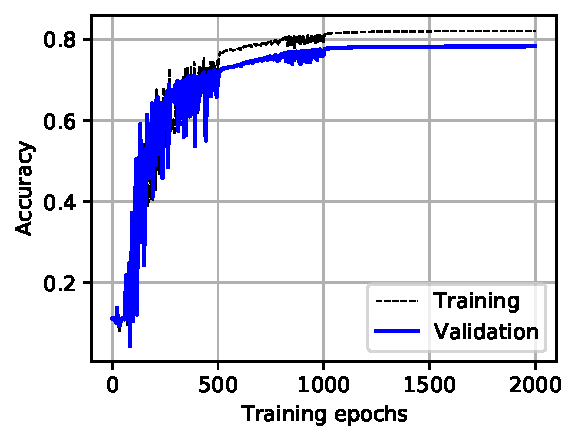
\includegraphics[width=0.23\textwidth]{python/accuracy_100_structures_adaptiveLR_CNN.pdf}}
	\quad
	\subfloat[][]{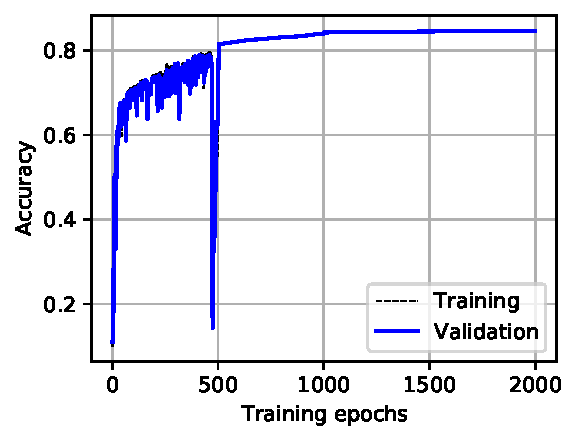
\includegraphics[width=0.23\textwidth]{python/accuracy_500_structures_adaptiveLR_CNN.pdf}}
	\\
	\subfloat[][]{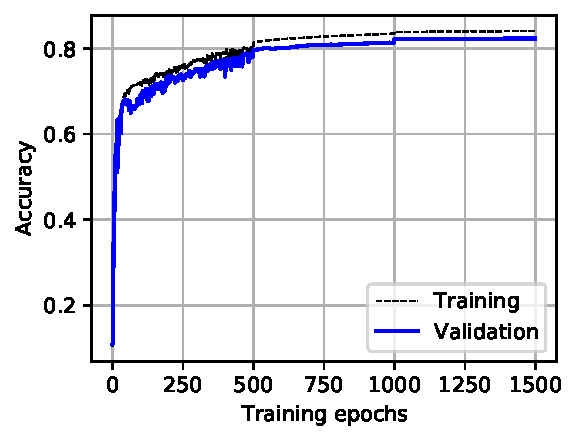
\includegraphics[width=0.23\textwidth]{python/accuracy_1000_structures_adaptiveLR_CNN.pdf}}
	\caption{Training and validation accuracy history for the best models of the 1D-\gls{cnn} hyperparameter optimization on (a): $ 100 $, (b): $ 500 $ and (c): $ 1000 $ structures after fine tuning the models with \gls{lrdecay} on the same datasets}
	\label{fig:accuracy_adaptiveLR_CNN}
\end{figure}

 The training histories of the \gls{tcn} fine tuning can be seen in Figure \ref{fig:accuracy_adaptiveLR_TCN}. The best model from the hyperparameter optimization on $ 1000 $ structures was not only fine tuned on $ 1000 $ structures but also on the full dataset of $ 9900 $ structures to see if any improvements can be realized when using much more training data (see Figure \ref{fig:accuracy_adaptiveLR_TCN} (d)). During the first phase of training with the highest learning rate there are strong oscillations of the accuracy for all the models. The first decrease of the learning rate helps to stabilize the training and for all the models gives a significant rise to the accuracy. In the later stages of the training all the models show a stable convergence. Only the model trained on $ 100 $ structures shows a bit of overfitting on the training dataset while the other models show no such signs. 

\begin{figure}[htp]
	\centering
	\subfloat[][]{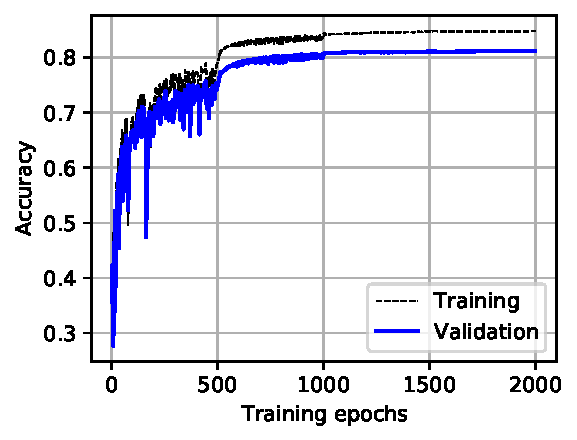
\includegraphics[width=0.23\textwidth]{python/accuracy_100_structures_adaptiveLR_TCN.pdf}}
	\quad
	\subfloat[][]{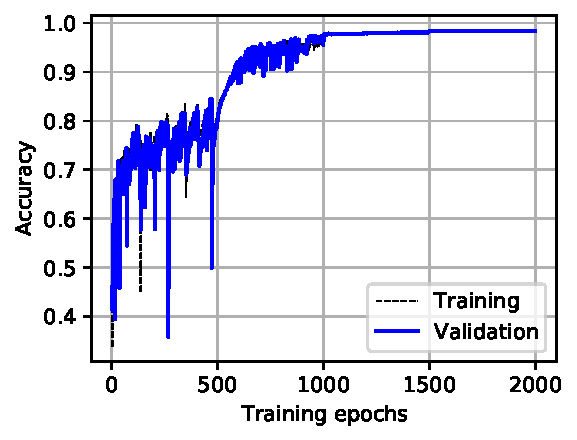
\includegraphics[width=0.23\textwidth]{python/accuracy_500_structures_adaptiveLR_TCN.pdf}}
	\\
	\subfloat[][]{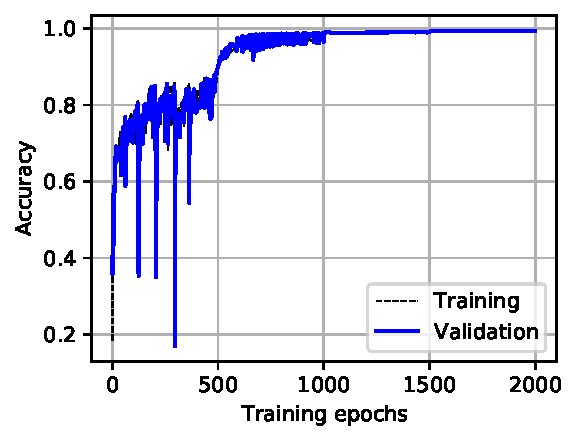
\includegraphics[width=0.23\textwidth]{python/accuracy_1000_structures_adaptiveLR_TCN.pdf}}
	\quad
	\subfloat[][]{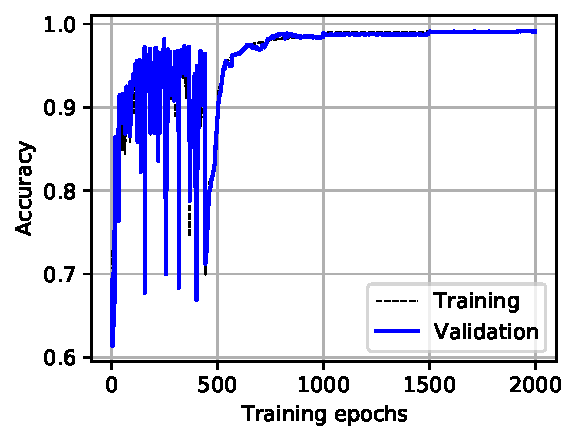
\includegraphics[width=0.23\textwidth]{python/accuracy_9900_structures_adaptiveLR_TCN.pdf}}
	\caption{Training and validation accuracy history for the best models of the \gls{tcn} hyperparameter optimization on (a): $ 100 $, (b): $ 500 $, (c): $ 1000 $ and (d): $ 9900 $ structures after fine tuning the models with \gls{lrdecay} on the same datasets}
	\label{fig:accuracy_adaptiveLR_TCN}
\end{figure}

\subsubsection{Model comparison}
\label{sec:model_comparison}

As a final validation all the fine tuned models are tested with the testing dataset of $ 100 $ structures. Table \ref{tab:accuracy_testing_rnn_cnn} shows an overview of the achieved accuracy for all \gls{rnn} (\gls{rnn}, \gls{lstm} and \gls{gru}) and \gls{cnn} models (1D-\gls{cnn} and \gls{tcn}).

It can be noticed that for \gls{rnn} models, the difference between the validation accuracy and the testing accuracy is notable. The networks have difficulties to generalize the patterns learned to new sets of data. But, as previously analysed in section \ref{sec:rnn_fine_tuning_results}, this could also be the result of the \gls{rul} classification which gives a larger bandwidth to the last classes and therefore leads to an imbalance of the training dataset towards the classes with higher \gls{rul} values. The testing dataset meanwhile focuses on the first classes, which are smaller. This imbalance leads to an increasing possibility of wrong predictions of the \gls{rul} on the testing dataset. One lead to explore would be to adapt the accuracy metric to take into account this imbalance of the training and testing data. Nonetheless, \glspl{gru} seem to work better on large datasets, reaching $ 97 \% $ validation accuracy when trained on  $ 1000 $ structures.

For the 1D-\gls{cnn} and \gls{tcn} models there is a steady increase in the achieved accuracy on the testing dataset if the amount of structures for training is increased. The increase in testing accuracy corresponds largely to the increase in validation accuracy. The testing accuracy is in the same order of magnitude as the validation accuracy indicating that the networks generalize well to new sets of data. In general \glspl{tcn} work better than 1D-\glspl{cnn}, especially on the larger datasets of $ 500 $ and $ 1000 $ structures where the \glspl{tcn} achieve close to $ 100 \% $ accuracy. When trained on the complete dataset of $ 9900 $ training structures the \gls{tcn} achieved $ 100 \% $ accuracy on the testing dataset.

\begin{table}[htp]
	\centering
	\caption{Accuracy of all fine tuned \gls{rnn} (\gls{rnn}, \gls{lstm} and \gls{gru}) and \gls{cnn} models (1D-\gls{cnn} and \gls{tcn}) on the validation and testing datasets}
	\label{tab:accuracy_testing_rnn_cnn}
	\setlength{\tabcolsep}{3pt} % Default value: 6pt
	\begin{tabular}{p{2.5cm}|lll|llll}
		Model type & \multicolumn{3}{c|}{1D-\gls{cnn}} & \multicolumn{4}{c}{\gls{tcn}} \\
		\hline
		Number of training structures & $ 100 $ & $ 500 $ & $ 1000 $ & $ 100 $ & $ 500 $ & $ 1000 $ & $ 9\,900 $ \\
		Validation accuracy & $ 0.78 $ & $ 0.84 $ & $ 0.82 $ & $ 0.81 $ & $ 0.98 $ & $ 0.99 $ & $ 0.99 $ \\
		Testing accuracy & $ 0.82 $ & $ 0.84 $ & $ 0.84 $ & $ 0.82 $ & $ 0.98 $ & $ 0.99 $ & $ 1.00 $ \\
		\multicolumn{8}{c}{}
	\end{tabular}

	\setlength{\tabcolsep}{2pt} % Default value: 6pt
	\begin{tabular}{p{2.5cm}|lll|lll|lll}
		Model type & \multicolumn{3}{c|}{\gls{rnn}} & \multicolumn{3}{c|}{\gls{lstm}} &  \multicolumn{3}{c}{\gls{gru}}\\
		\hline
		Number of training structures & $ 100 $ & $ 500 $ & $ 1000 $ & $ 100 $ & $ 500 $ & $ 1000 $ & $ 100 $ & $ 500 $ & $ 1000 $ \\
		Validation accuracy & $ 0.90 $ & $ 0.91 $ & $ 0.89 $ & $ 0.85 $ & $ 0.93 $ & $ 0.93 $ & $ 0.78 $ & $ 0.96 $ & $ 0.97 $ \\
		Testing accuracy & $ 0.84 $ & $ 0.90 $ & $ 0.78 $ & $ 0.73 $ & $ 0.83 $ & $ 0.72 $ & $ 0.70 $ & $ 0.77 $ & $ 0.75 $
	\end{tabular}

\end{table}

\section{Conclusions and outlook}
\label{sec:conclusions_outlook}

The aim of this study to predict the \gls{rul} of pre cracked plates based on strain gauges data with Deep Learning methods could be achieved. All investigated models were successfully trained on the available dataset and achieved an accuracy of at least $ 70 \% $ on the testing dataset. It usually was the case that more available training data lead to a better performance of the models. The best performance in general was achieved by \gls{tcn} models. Confirming the good results with \glspl{tcn} of other researchers like Bai et al. \cite{Bai2018} and Li et al. \cite{Li2018}. This result again questions the general practice to use \gls{rnn} models as the first choice for time series prediction while \gls{cnn} models should be used for image classification and related tasks. The \gls{tcn} models when trained on more than $ 500 $ structures achieved closed to $ 100 \% $ accuracy confirming their excellent suitability to time series prediction problems.

The \gls{rnn} models, especially the \glspl{gru}, achieved good performances on the validation dataset while when tested on the testing dataset there is a significant drop in performance. This might be the result of the testing dataset being focused on short \gls{rul} values close to failure of the plates. In this area there are many different \gls{rul} classes because of the parabolic distribution of the class boundaries. The \glspl{gru} seem to have troubles generalizing to this area while they might work very well on the classes with bigger \gls{rul} values. Thus, a lead to explore would be a hybrid model combining a \gls{gru} and \gls{tcn} architecture, to improve learning of the different patterns in the data.

The in general good results achieved on this dataset should come at no surprise as the dataset is synthetic without the flaws of real world data. There is no noise in the data which would never be the case in reality. The virtual strain gauges are always placed at the exact same location on the plates while in reality there is always a position tolerance when placing them on a structure. The synthetic dataset can also provide the models with amounts of data which are not available in reality. Especially the amount of data available until the \gls{eol} of the structures.

Fur further research it is important to train and test the models on noisy data and focus on improving their accuracy when trained on smaller datasets, e.g. on $ 100 $ structures. This smaller datasets should also include less data towards the \gls{eol} of the structures.

Right now the models are restricted to a fixed sliding window size. They therefore can not use less but also not more of the available data than dictated by the sliding window size. A possible solution to consider for this problem would be to use a much larger sliding window together with zero padding when not enough data to fill the window is available. This way the networks could use all of the available past and current data independently of the sliding window size and the length of the currently available time series of the structure.

%\newpage
\printbibliography

\end{document}